\chapter{Design og implementasjon av et skytilkoblet pulsoksimeter}
\label{ch:implementation1}

Kapittelet beskriver hvordan en prototype av et skytilkoblet pulsoksimeter med innebygget autentisering ble utviklet.
Første del av kapittelet handler om valg av teknologien før blabla
Siste del av kapittelet går mer detaljert inn i utviklingen av prototypen, med delkapitlene
\textit{Implementasjon av klientkomponenter} og \textit{Implementasjon av skytilkobling}.

\section{Designkrav til prototype}

\begin{enumerate}
    \item [\textbf{FK1}] Når brukeren trykker på knappen skal systemet sette i gang en måling
        \begin{enumerate}
          \item [\textbf{FK1.1}] Brukeren må legge fingeren på fingeravtrykksensoren for å autentisere innen 10 sekunder.
          \item [\textbf{FK1.2}] Ved vellykket autentisering skal brukeren få 120 sekunder til å gjennomføre
              en måling.
          \item [\textbf{FK1.3}] Brukeren starter målingen ved å stikke fingeren inn i pulsoksimeteret.
              En måling er definert som kontinuerlig datainnhenting i 20 sekunder.
          \item [\textbf{FK1.4}] Systemet skal sende data fra målingen kontinuerlig til en skytjeneste.
          \item [\textbf{FK1.5}] Når en måling er ferdig, skal skjermen på pulsoksimeteret og lysdiodene indikere til brukeren
              at det er godkjent.
          \item [\textbf{FK1.6}]Systemet skal vise rødt lys og sende brukeren tilbake til sovende modus dersom et av de
              foregående kravene ikke oppfylles.
        \end{enumerate}
    \item [\textbf{FK2}] Når brukeren holder inne knappen i over fire sekunder og slipper i utviklingsmodus,
        skal prosessen for å registrere et fingeravtrykk settes i gang.
        \begin{enumerate}
          \item [\textbf{FK2.1}] Registreringen blir gjort sammen med helsepersonell som forklarer hva som skal gjøres.
          \item [\textbf{FK2.2}] Dersom noe går galt under registreringen, skal systemet vise rødt lys og sende brukeren
              tilbake til sovende modus igjen.
        \end{enumerate}
\end{enumerate}

% Use case
% Scenarie
% Stegene

\section{Beskrivelse av prototype}
Prototypen bestod av følgende komponenter:

\begin{itemize}
  \item Raspberry Pi Zero W
  \item GT-511C3 (fingeravtrykksensor)
  \item Nonin 3230 (pulsoksimeter med \gls{ble})
  \item Standard trykknapp
  \item Tre RGB-lysdioder og én hvit lysdiode
  \item 3D-printet hus
\end{itemize}

Komponentene ble presentert i forrige kapittel. Raspberry Pi Zero W ble valgt som prototypeplattform istedenfor
alternativer som Tessel 2 og Arduino Yún. Det var et ønske om å bruke JavaScript og Node.js som utviklingsmiljø, og Arduino
bruker C/C++ som utviklingsspråk. Tessel 2 er en prototypeplattform basert på Node.js, men har få konfigurasjonsmuligheter
og \gls{ble} er ikke innebygget.

Prototypen bestod av to deler, en klientsideløsning og en serverløsning.
Oversikt over klientsideløsningen med hvordan komponentene kommuniserte med Raspberry Pi er i figur \ref{fig:prototypeoversikt}.
\begin{figure}
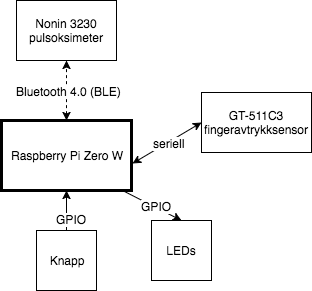
\includegraphics[width=0.55\textwidth, center]{fig/prototype/oversiktlosning}
\caption{Sammenhengen mellom de ulike komponentene}
\label{fig:prototypeoversikt}
\end{figure}

Klientsideløsningen ble utviklet rundt
et Nonin 3230-pulsoksimeter utlånt av Trondhem kommune. Den kjørte på Node.js, en kryssplattform JavaScript-runtime som bruker den
samme JavaScript-motoren som Chromium (V8). Løsningen bestod av én hovedapplikasjon, og en tilhørende modul hver for henholdsvis fingeravtrykksensoren,
pulsoksimeteret og knapp/lysdioder. Disse modulene er utdypt nærmere i neste delkapittel, \textit{Implementasjon av klientkomponenter}.
Koden til hovedmodulen er i vedlegg TODO.

Applikasjonen startet automatisk opp på Raspberry Pi, og loggførte alle hendelser til en tekstfil.
Prototypen sendte IP-adressen sin ved oppstart slik at det var mulig å nå den utenfra.
Klientsiden snakket med serveren over MQTTS, og ble autentisert med et sertifikat. Sensordataen fra pulsoksimeteret ble publisert til
AWS IoT dersom brukeren var autentisert med fingeravtrykksensor. Virkemåten til prototypen var den samme som det de funksjonelle
kravene spesifiserte i kapittel \ref{ch:requirements}. Se figur TODO for et bilde av hvordan prototypen ble seende ut.

Serveren, som var basert på AWS IoT, hadde en
regel for å prosessere dataen som kommer inn. Denne regelen sendte dataen videre til en lambdafunksjon som puttet dataen
i InfluxDB, en tidsseriedatabase. Denne databasen ble knyttet opp mot Grafana, et åpent kildekode-verktøy som integrerer
med InfluxDB og viste fram grafer og metrikker i ulike konfigurerbare \textit{dashboards}. En arkitekturoversikt over løsningen
kan finnes i figur TODO. Serverløsningen er videre utdypt i delkapittel \ref{sec:implementasjon_skytilkobling}.

\section{Implementasjon av klientkomponenter}

\subsection{Trykknapp og lysdioder}
Figur \ref{fig:breadboard} viser hvordan trykknappen og lysdiodene ble koblet på
portene til Raspberry Pi med et \textit{breadboard}. Oppkoblingen er logisk ekvivalent med prototypen.
I selve prototypen ble to RGB-lysdioder og en knapp loddet fast med motstander på et et lite brett av Terje Røsand (se figur \ref{fig:brett}).
Koblingsskjemaet er i figur \ref{fig:schematics}. Alle komponentene delte felles jord.

\begin{figure}
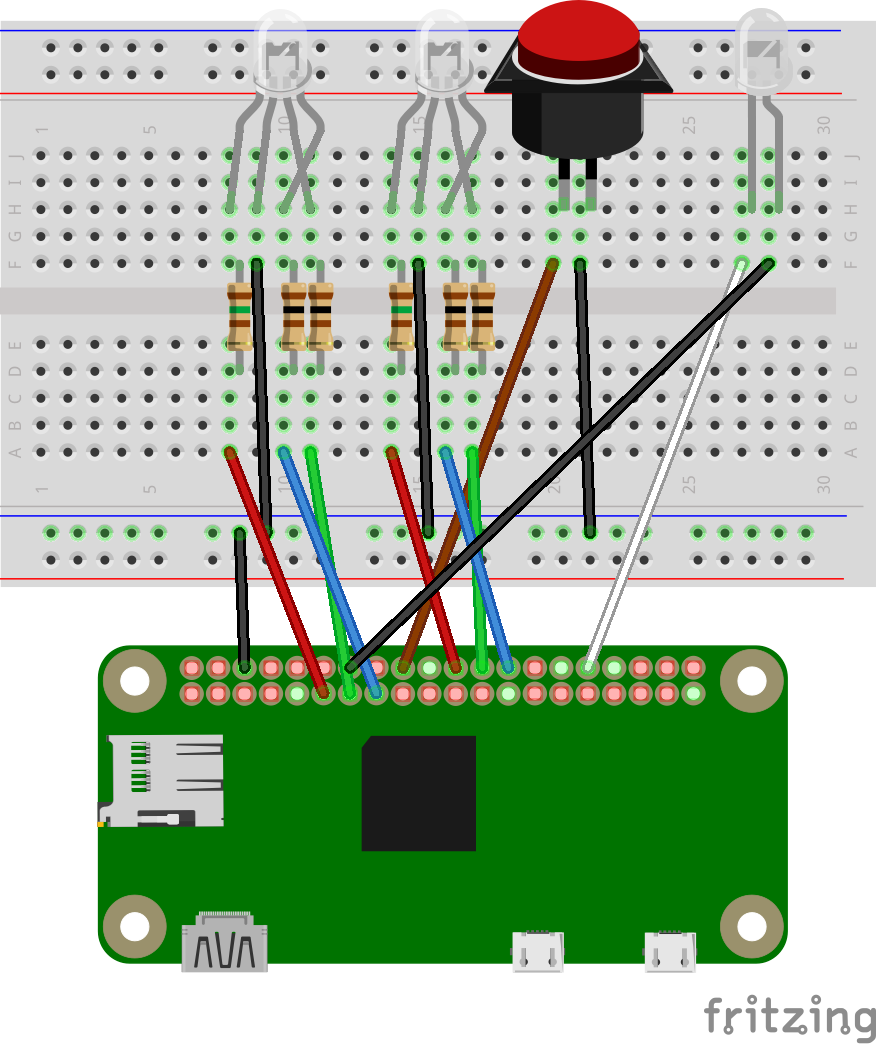
\includegraphics[width=0.75\textwidth, center]{fig/prototype/breadbord}
\caption{Oppkobling av trykknapp og lysdioder}
\label{fig:breadboard}
\end{figure}

\begin{figure}
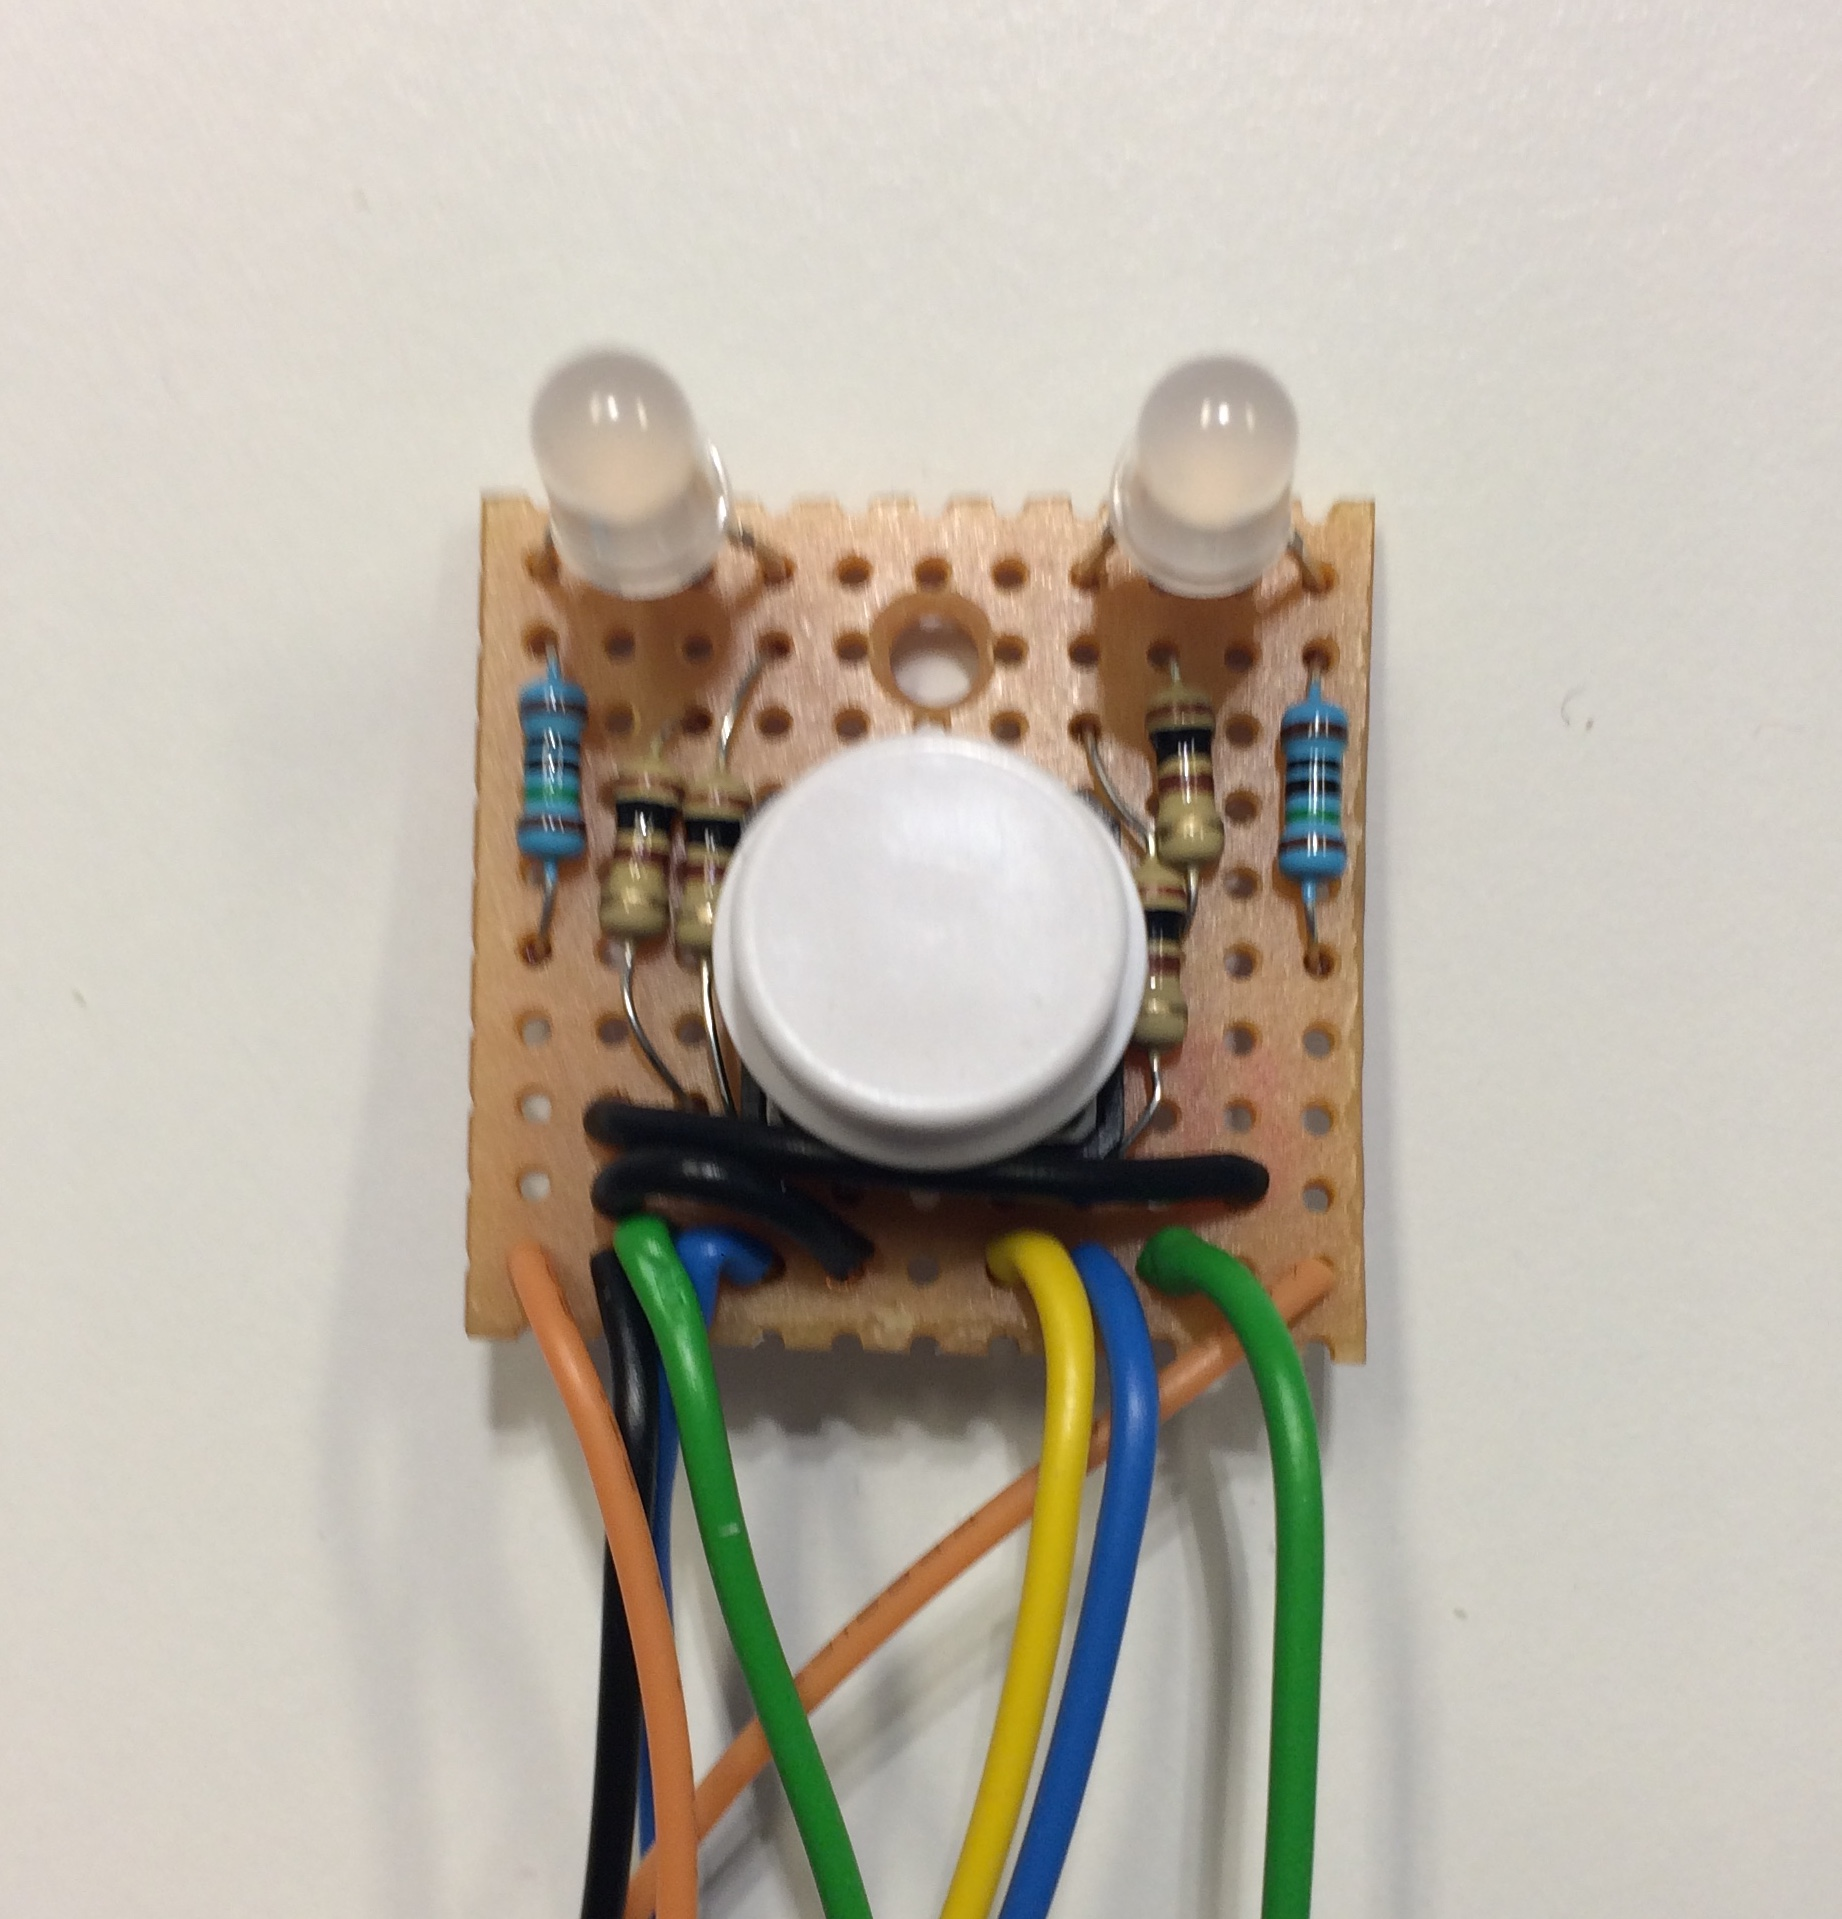
\includegraphics[width=0.65\textwidth, center]{fig/prototype/ekte_knappleds}
\caption{Oppkobling av trykknapp og lysdioder på brett}
\label{fig:brett}
\end{figure}

\begin{figure}
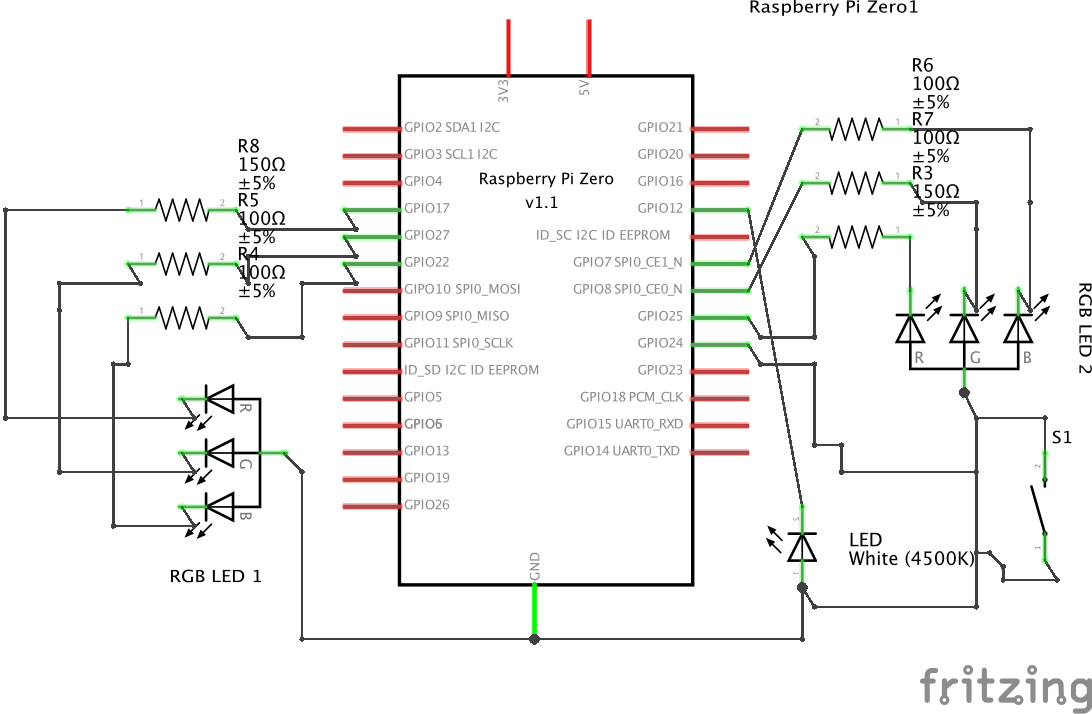
\includegraphics[width=0.95\textwidth, center]{fig/prototype/schmeatic}
\caption{Koblingsskjema av trykknapp og lysdioder}
\label{fig:schematics}
\end{figure}

For å gjøre håndteringen av knapp og lysdioder enklere, ble det utviklet et lite JavaScript-bibliotek.
Koden til dette biblioteket er lagt ved i tillegg \ref{appendix:pigpio-components}. Kodesnutt
\ref{lst:pigpio-components-usage} er et eksempel på bruk av dette biblioteket med den samme oppkoblingen som i
figur \ref{fig:breadboard}.

\begin{lstlisting}[frame=single, language=JavaScript,
    caption=Bruk av pigpio-components, label=lst:pigpio-components-usage]
const button = new Button({ gpio: 24, isPullup: true });
const rgbLed1 = new RGBLed({ red: 25, green: 8, blue: 7 });
const rgbLed2 = new RGBLed({ red: 17, green: 27, blue: 22 });
const whiteLed = new Led(12);

button.on('click', () =>
  console.log('press and release within 500 ms'));
whiteLed.on();
rgbLed1.color('blue').on();
rgbLed2.color('#DC143C').strobe();
\end{lstlisting}

\subsection{GT-511C3}
Koden til fingeravtrykksensoren ble utviklet som en tynn abstraksjon over \gls{npm}-biblioteket \textit{GT-511C3}
\footnote{\url{https://github.com/the-AjK/GT-511C3}}, utgitt under BSD-3-lisens. Implementasjonen ligger
i filen \textit{index.js} i modulen \textit{fingerprint}
\footnote{\url{https://github.com/andybb/smart-pulse-oximeter/blob/master/fingerprint/index.js}}.
Denne modulen eksporterer to metoder: \textit{enrollFingerAndRetrieveTemplate} og \textit{setFingerprintTemplateAndVerify}.

Den første metoden går igjennom prosessen for å legge til et fingeravtrykk i databasen til sensoren, og henter ut et avtrykk
på 498 bytes. Dette avtrykket kan og bør lagres i en skytjeneste, men dette ble ikke implementert i prototypen.
Den andre metoden har støtte for å ta inn et slikt avtrykk, og legge det inn i databasen til sensoren før avtrykket
verifiseres ved å legge riktig finger på sensoren. I prototypen ble det antatt at avtrykket lagres på samme sted i databasen hver gang.

Fingeravtrykksensoren ble koblet til GPIO14 (TX) og GPIO15 (RX) som har seriell kommunikasjon. Sensoren ble også koblet til jord
og 5V for strøm. Ut av boksen støtter ikke Raspberry Pi Zero W seriell kommunikasjon fordi Bluetooth opptar den serielle porten.
Derfor ble \textit{mini-uart} slått på (fotnote). Dette er en seriell port med mindre hastighet knyttet til CPU-frekvensen.

\subsection{Nonin 3230}
Utgaven av Nonin 3230 Trondheim kommune har kjøpt inn bruker en proprietær Bluetooth-tjeneste med 128-bit \gls{uuid}.
I nyere utgaver kan man også bruke den åpne spesifikasjonen til \textit{Bluetooth SIG Pulse Oximeter Service}.
Den proprietære tjenesten heter \textit{Nonin Oximetry Service} og har \gls{uuid} \textit{46a970e00d5f11e28b5e0002a5d5c51b}.
Tjenesten har to karakteristikker -- \textit{Nonin Oximetry Measurement} som sender data hvert sekund som spesifiert
i tabell \ref{table:nonin-datapacket} og \textit{Nonin Control Point} som kan brukes til å synkronisere skjermen,
indikere at en måling er ferdig, eller sette sikkerhetsmodus. 

Et \gls{npm}-biblotek (fotnote url) kalt \textit{nonin-3230-ble} ble utviklet for å gjøre integrasjonen mot sensoren enklere.
Biblioteket baserer seg på \textit{noble-device} (fotnote), og inneholder metoder for å oppdage et pulsoksimeter,
koble til, lytte etter ny sensordata og indikere at en måling er ferdig. Sensordata kommer som et JavaScript-objekt
og inneholder teller, pulsfrekvens, SpO2 og et statusobjekt (se tabell \ref{table:nonin-status}).
Koden er lagt ved i appendiks \ref{lst:nonin-3230-library}.
Eksempel på bruk kan finnes i kodesnutt \ref{lst:nonin-3230-usage}.

Koden slik den er i dag er lagt opp til å utføre kontinuerlige målinger hvor sensordata mottas hvert sekund. Pulsoksimeteret
har også støtte for å utføre en spot-måling, det vil si én god måling som er kvalitetssikret av sensoren. Trondheim kommune
bruker kun spot-målinger i sin løsning i dag.

\begin{minipage}{\linewidth}
\begin{lstlisting}[frame=single, language=JavaScript,
    caption=Bruk av nonin-3230-ble, label=lst:nonin-3230-usage]
const Nonin3230 = require('nonin-3230-ble');

Nonin3230.discover((pulseOximeter) => {
  pulseOximeter.connectAndSetup((error) => {
    if (error) {
      console.error(error);
    }
    let counter = 0;
    // receive a new measurement every second
    pulseOximeter.on('data', (data) => {
      // data: { counter: int, pulseRate: int, oxygenSaturation: int, status: object }
      counter++;
      if (counter > 15) {
        pulseOximeter.stopMeasurement(() => console.log('Stopped'));
      }
    });
  });
});
\end{lstlisting}
\end{minipage}

Kildekoden er åpen og kan kjøres fra alle enheter som har støtte for Node og \gls{ble}.


\begin{table}[]
\centering
\begin{tabular}{|l|l|l}
\hline
\multicolumn{3}{|l|}{\textbf{Datapakke til pulsoksimeter}} \\ \hline
\textbf{Byte} & \textbf{Felt} & \multicolumn{1}{l|}{\textbf{Beskrivelse}} \\ \hline
1 & Lengde & Antallet bytes inkludert denne. \\ \hline
2 & Status & \multicolumn{1}{l|}{Indikerer nåværende enhetsstatus (tabell \ref{table:nonin-status}).} \\ \hline
3 & Batterispenning & \multicolumn{1}{l|}{Spenningsnivået til batteriene som brukes.} \\ \hline
4-5 & \begin{tabular}[c]{@{}l@{}}Perfusjonsindeks\\ (PI)\end{tabular} & \multicolumn{1}{l|}{PI = AC/DC*100\%} \\ \hline
6-7 & Teller & \multicolumn{1}{l|}{\begin{tabular}[c]{@{}l@{}}Verdien økes hvert sekund (0-65535). Kan bli brukt\\ til å sjekke at det ikke er noe datatap.\end{tabular}} \\ \hline
8 & SpO2 & \multicolumn{1}{l|}{SpO2-prosent, 0-100 (gjennomsnitt av fire slag).} \\ \hline
9-10 & Pulsfrekvens & \multicolumn{1}{l|}{\begin{tabular}[c]{@{}l@{}}Pulsfrekvens i slag per minutt, 0-321\\ (gjennomsnitt av fire slag).\end{tabular}} \\ \hline
\textgreater11 & Reservert & \multicolumn{1}{l|}{Reservert til fremtidig bruk} \\ \hline
\end{tabular}
\caption{Nonin 3230: Format på datapakke ref: nonin integration guide}
\label{table:nonin-datapacket}
\end{table}

\begin{table}[]
\centering
\begin{tabular}{|l|l|l}
\hline
\multicolumn{3}{|l|}{\textbf{Statusfelt (aktiv høy)}} \\ \hline
\textbf{Bit} & \textbf{Felt} & \multicolumn{1}{l|}{\textbf{Beskrivelse}} \\ \hline
7 & Reservert & Reservert til fremtidig bruk. \\ \hline
6 & Kryptering & \multicolumn{1}{l|}{\begin{tabular}[c]{@{}l@{}}1 = tilkoblingen er kryptert\\ 2 = tilkoblingen er ikke kryptert\end{tabular}} \\ \hline
5 & Lavt batteri & \multicolumn{1}{l|}{Batterinivået er lavt. Bytt batteri.} \\ \hline
4 & CorrectCheck & \multicolumn{1}{l|}{\begin{tabular}[c]{@{}l@{}}1 = OK\\ 2 = Plasser fingeren lengre inn i enheten\end{tabular}} \\ \hline
3 & Søker & \multicolumn{1}{l|}{Oksimeteret søker etter etterfølgende pulssignaler.} \\ \hline
2 & SmartPoint & \multicolumn{1}{l|}{\begin{tabular}[c]{@{}l@{}}Brukt til å indikere at dataen har bestått SmartPoint-\\ algoritmen.\end{tabular}} \\ \hline
1 & Lavt/svakt signal & \multicolumn{1}{l|}{\begin{tabular}[c]{@{}l@{}}Styrken til pulssignalet er 0,3 \% modulasjonsgrad\\ eller mindre.\end{tabular}} \\ \hline
0 & \begin{tabular}[c]{@{}l@{}}Indikering av\\ skjermsynkronisering\end{tabular} & \multicolumn{1}{l|}{\begin{tabular}[c]{@{}l@{}}Indikerer at skjermen er synkronisert med\\ innsamleren av data.\end{tabular}} \\ \hline
\end{tabular}
\caption{Nonin 3230: Format på statusfeltet til datapakke ref: nonin integration guide}
\label{table:nonin-status}
\end{table}

\subsection{3D-printet hus}
Det 3D-printede huset til prototypen ble designet og printet ut av Terje Røsand basert på alle komponentstørrelsene i samarbeid
med Andreas Drivenes. Å integrere pulsoksimeteret i huset var den mest utfordrende delen av designet, og det gjorde at det ikke var
mulig å få plass til noen andre komponenter over denne sensoren. Alle de andre sensorene måtte plasseres til høyre for pulsoksimeteret.
Huset bestod av to uliker deler som klikkes sammen. Figur \ref{fig:3dmodell_topp1}
og figur \ref{fig:3dmodell_topp2} viser toppdelen, og figur \ref{fig:3dmodell_bunn} viser bunndelen.

Pulsoksimeteret og brettet med lysdioder og knapp ble skrudd fast med tre skruer til toppdelen. Pulsoksimeteret ble presset mot toppdelen
med et innlagt, mykt materiale. Raspberry Pi Zero W ble skrudd fast med fire skruer til bunndelen.

\begin{figure}
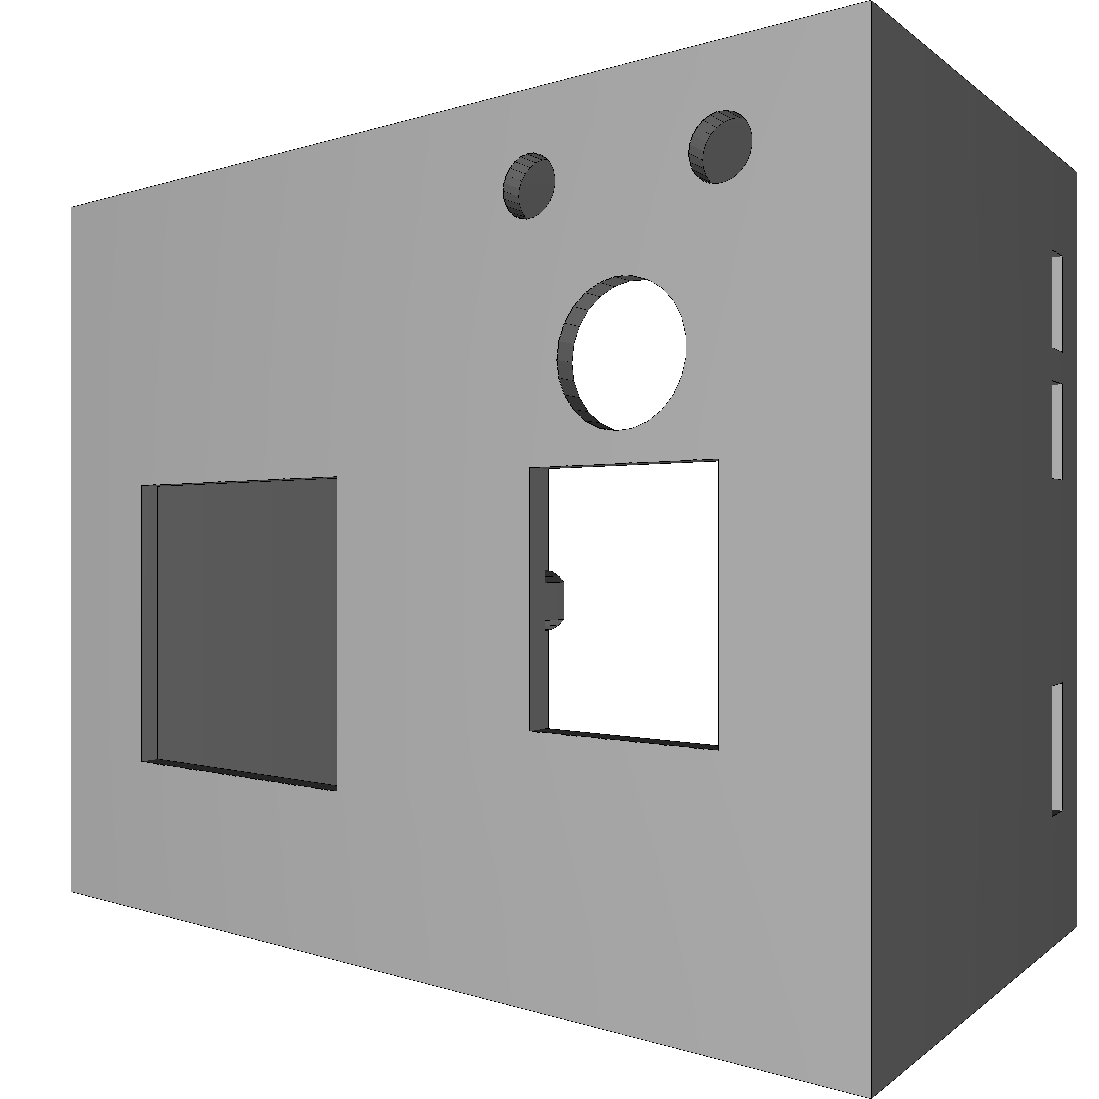
\includegraphics[width=0.65\textwidth, center]{fig/prototype/hoved_fra_topp}
\caption{3D-modell av prototype: Topp}
\label{fig:3dmodell_topp1}
\end{figure}
\begin{figure}

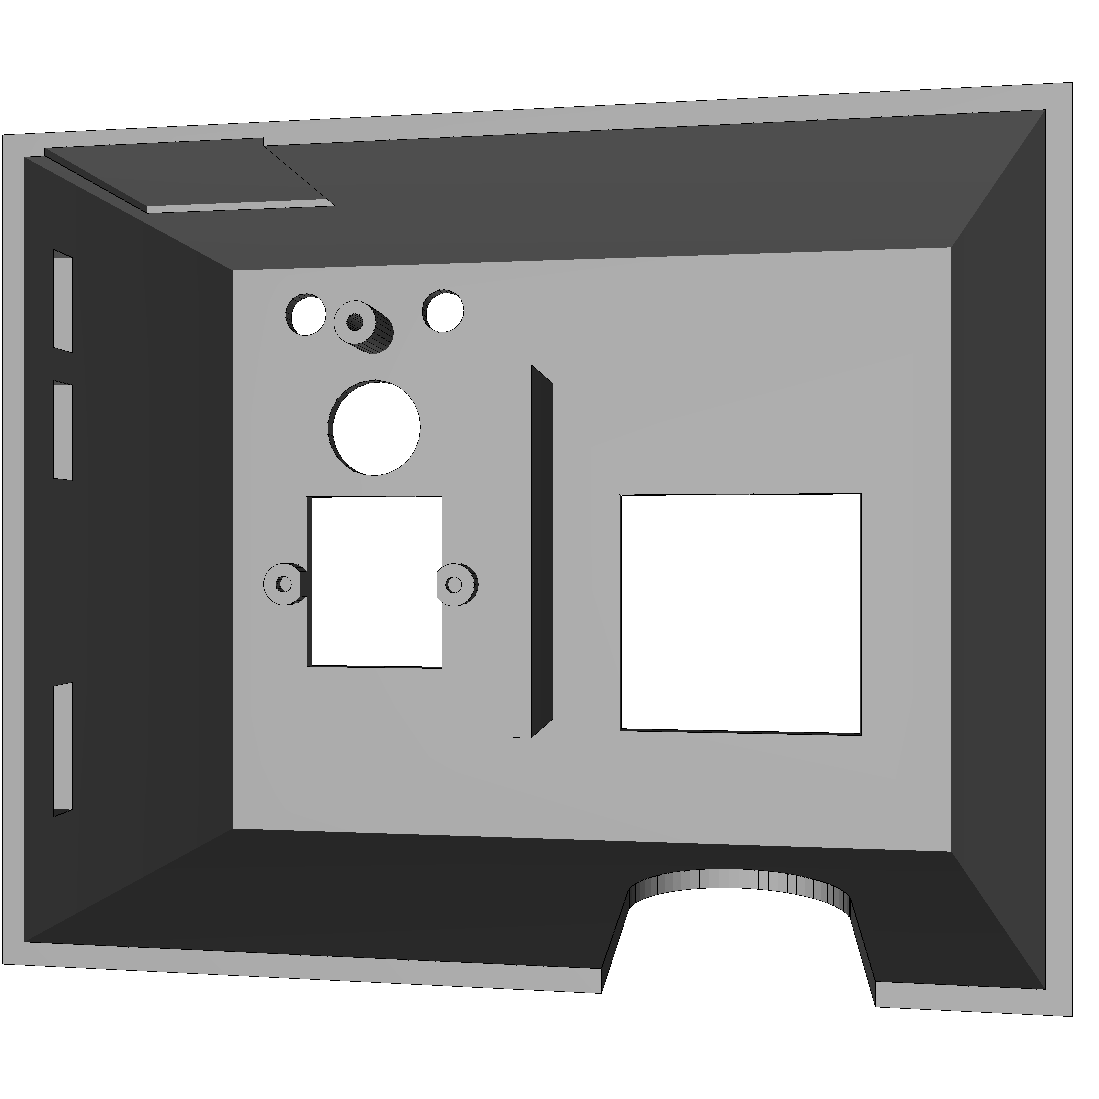
\includegraphics[width=0.65\textwidth, center]{fig/prototype/hoved_frabunn}
\caption{3D-modell av prototype: Topp, sett fra bunn}
\label{fig:3dmodell_topp2}
\end{figure}

\begin{figure}
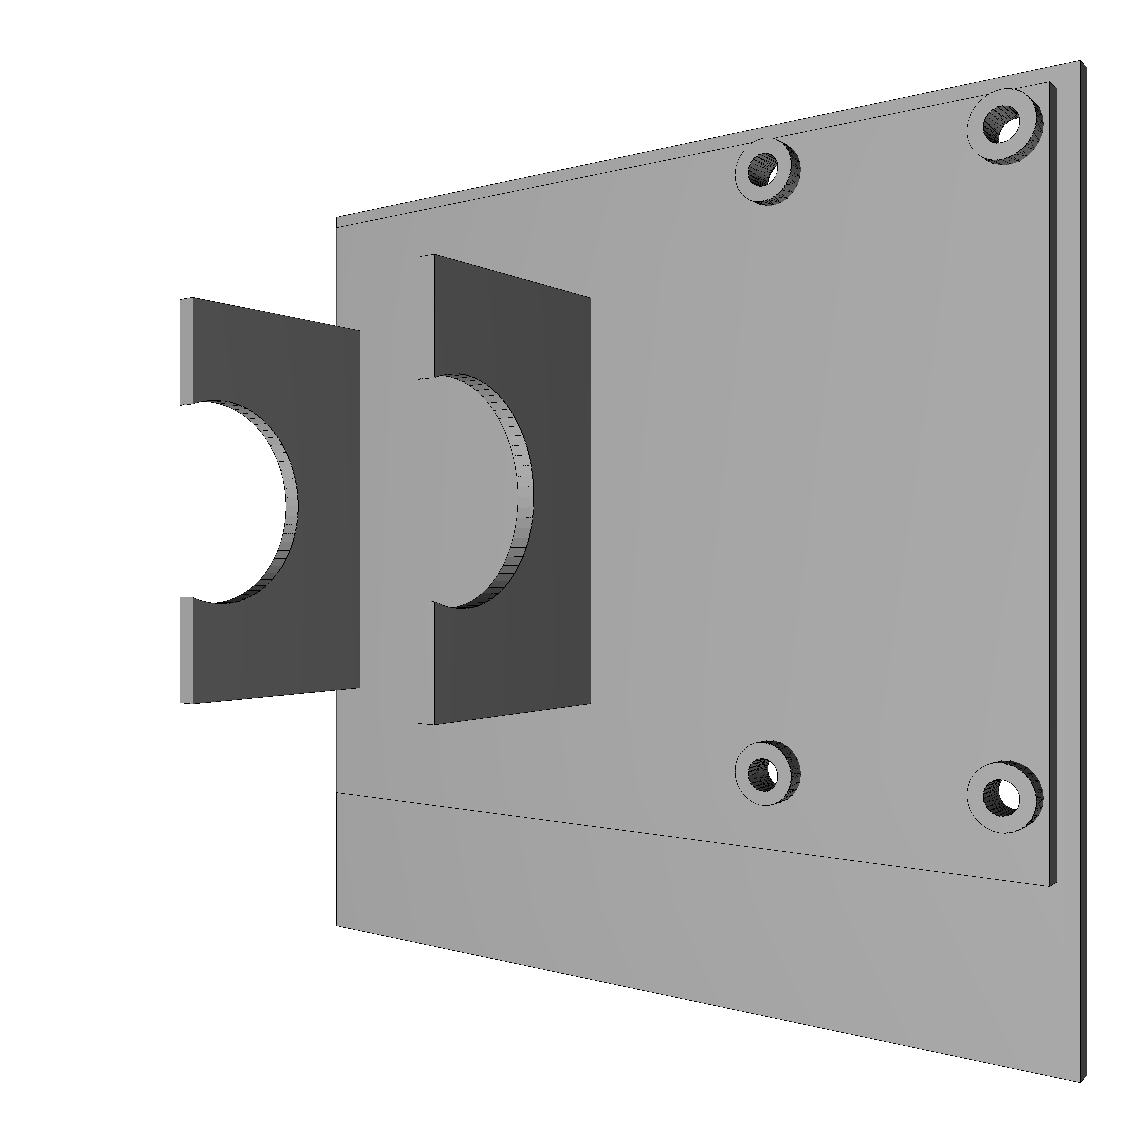
\includegraphics[width=0.65\textwidth, center]{fig/prototype/bunn_fratopp}
\caption{3D-modell av prototype: Bunn}
\label{fig:3dmodell_bunn}
\end{figure}

\section{Implementasjon av skytilkobling}
\label{sec:implementasjon_skytilkobling}

\subsection{Registrering og oppkobling til AWS IoT}
Som beskrevet i delkapittel \ref{sec:aws_iot}, må en enhet registreres i thing registry i AWS IoT og
få tilknyttet et sertifikat for å fungere. Kodesnutt \ref{lst:aws_register} viser hvordan prototypen ble registrert
hos AWS IoT med kommandolinjeverktøyet de tilbyr. Andre muligheter hadde vært å bruke webgrensesnittet eller
gjort det programmatisk med REST API-et.

Kommandoen på linje 2 i kodesnutt \ref{lst:aws_register} genererte et X.509-sertifikat og et 2048-bit RSA nøkkelpar.
Den printet ut et Amazon Resource Number (ARN) og en id som hører til sertifikatet,
sertifikatsdataen og det genererte nøkkelparet (assymetrisk). Sertifikatet ble satt til å være aktivt.
Det er også mulig å registrere egne sertifikater fra en egen sertifikatutsteder.

En policy trengs for at prototypen skal godkjennes av AWS IoT. Policy er et JSON-dokument med flere
\textit{statements} som inkluderer feltene \textit{effect}, \textit{action} og \textit{resource}.
Policyen til prototypen ble laget på linje 3 i kodesnutt \ref{lst:aws_register}, og kan sees i kodesnutt \ref{lst:aws_policy}.
Denne policyen var veldig lite restriktiv og tillot alle actions (connect, publish, subscribe, get/modify thing shadow) på hvilken
som helst resource. En mer restriktiv policy hadde vært mer relevant om prototypen skulle blitt satt i produksjon.

De to siste kommandoene knyttet henholdsvis sertfikatet til tingen, og policyen til sertifikatet. Dette gjorde at man kunne autentisere prototypen
basert på sertifikatet.

\begin{lstlisting}[frame=single, language=bash, caption=Registrere en ting i AWS IoT, label=lst:aws_register]
aws iot create-thing --thing-name "smart-pulse-oximeter"
aws iot create-keys-and-certificate --set-as-active
aws iot create-policy --policy-name "smart-pulse-oximeter-Policy" --policy-document "file://policy.json"
aws iot attach-thing-principal --thing-name "smart-pulse-oximeter" --principal "[sertifikats-ARN generert paa linje 2]"
aws iot attach-principal-policy --principal "[sertifikats-ARN generert paa linje to]" --policy-name "smart-pulse-oximeter-Policy"
\end{lstlisting}

\begin{lstlisting}[language=JavaScript, frame=single,
    caption=Policy-dokument (policy.json), label=lst:aws_policy]
{
  "Version": "2012-10-17",
  "Statement": [
    {
      "Effect": "Allow",
      "Action": [
        "iot:*"
      ],
      "Resource": [
        "*"
      ]
    }
  ]
}
\end{lstlisting}

For å koble klientsiden av prototypen til AWS IoT, ble nøklene og sertifikatet generert over brukt.
AWS IoT autentiserer prototypen basert på tingnavnet, nøklene og sertifikatet.
Se kodesnutt \ref{lst:aws_connect}.
%\lstset{
%   aboveskip=20pt, belowskip=20pt,
%   numbers=left
% }
\begin{lstlisting}[language=JavaScript, frame=single,
    caption=Koble prototype til AWS IoT, label=lst:aws_connect]
const awsIot = require('aws-iot-device-sdk');

const device = awsIot.device({
  keyPath: process.env.AWS_KEY_PATH,
  certPath: process.env.AWS_CERT_PATH,
  caPath: process.env.AWS_CA_PATH,
  clientId: 'smart-pulse-oximeter',
  region: 'eu-central-1'
});

device.on('message', (topic, payload) => { 
  // do something with payload
});
device.subscribe('oximetry');

// Pretend like we have got an object called 'oximetry' from the pulse oximeter
device.publish('oximetry', JSON.stringify({ oximetry }));
\end{lstlisting}

\subsection{Oppsett av businessregler og visning av data}

\begin{lstlisting}[frame=single, language=bash, caption=Sette opp en businessregel i AWS IoT, label=lst:aws_business]
aws iot create-topic-rule --rule-name "smart-pulse-oximeter-Rule" --topic-rule-payload "file://payload.json"

//payload.json mock:
const payload =
{
  "sql": "SELECT * from 'oximetry'",
  "description": "Send data from pulse oximeter to a database and viewing tool",
  "actions": [
    {
      "lambda": {
        "functionArn": "[ARN of lambda function]"
      }
    }
  ],
  "ruleDisabled": false,
  "awsIotSqlVersion": "2016-03-23"
};
\end{lstlisting}

\textbf{TODO:} Her kommer det litt mer om lamdafunksjon og visning av data fra en database
